\section{Forces}

\subsection{Force \& potential energy in 1D}

Consider a mass $m$ moving in a straight line with position $x(t)$. Suppose the force \textit{only} depends on $x$.
\begin{definition}[Potential energy]
    Define \textit{potential energy} $ V(x) $ as 
    \[
        F(x) = -\frac{\mathrm{d}V}{\mathrm{d}x} \Longrightarrow V(x) = \int^{x}F(x')\dd x.
    \]
\end{definition}

The equation of motion is
\[
    m \ddot{x}=-\frac{\mathrm{d}V}{\mathrm{d}x} .
\]

\begin{definition}[Kinetic energy]
    $T=\frac{1}{2}m \dot{x}^2$, generalised as $ T=\frac{1}{2}m|\dot{\bfx}|^2 $. 
\end{definition}
\begin{definition}[Total energy]
    $ E=T+V = \frac{1}{2}m \dot{x}^2+V(x) $.
\end{definition}
\begin{proposition}
    The total energy is conserved. That is, 
    \[
        \frac{\mathrm{d}E}{\mathrm{d}t}=0. 
    \]
\end{proposition}
\begin{proof}
    Remind that $F$ \textit{only} depends on position $x$.
    \begin{align*}
        \frac{\mathrm{d}E}{\mathrm{d}t} &= \frac{\mathrm{d}}{\mathrm{d}t}\left( \frac{1}{2} m \dot{x}^2+V(x) \right) = m \dot{x} \ddot{x} + \frac{\mathrm{d}V}{\mathrm{d}x} \dot{x}\\
        &= \dot{x} \left( m \ddot{x} + \frac{\mathrm{d}V}{\mathrm{d}x}  \right) = 0.
    \end{align*}
\end{proof}

\begin{note}
    For conservation of $ \frac{1}{2} m \dot{x}^2 + \Phi $ we require 
    \[
        \dot{x}F = -\frac{\mathrm{d}\Phi}{\mathrm{d}t}. 
    \]
    In principle $ \Phi $ may depend on $ x, \dot{x}, t $. It is usually the case that there is no such $ \Phi $ if $F$ depends on $ \dot{x} $ and/or $t$.
\end{note}

\begin{example}[Harmonic oscillator]
    $ F=-kx $. Then 
    \[
        V(x) = - \int^{x} -kx' \,\mathrm{d}x' = \frac{1}{2}k x^2,\text{ wlog}.
    \]
    Since $ m \ddot{x} = -kx $, $ x(t) = A \cos \omega t+B \sin \omega t $ and $ \dot{x}(t) = -\omega A \sin \omega t+\omega B \cos \omega t $ for suitable constant $ A,B $ and $ \omega=\sqrt{k/m} $.

    Can check $E$ is indeed conserved.
\end{example}

\subsubsection*{Quantitative insight}
In 1D conservation of energy gives useful information about motion. Conservation of energy is a 1st integration of Newton's 2nd law. Since 
\[
    E= \frac{1}{2}m \dot{x}^2 + V(x) \Longrightarrow \dot{x} = \pm \sqrt{\frac{2}{m}(E-V(x))},
\]
we can use this to derive $x$:
\[
    \pm \int_{x_0}^{x} \frac{\mathrm{d}x'}{\sqrt{\frac{2}{m}(E-V(x'))}} = t-t_0.
\]
This is an implicit solution for $x(t)$. In principle we can evaluate the integral and find $x(t)$.

\subsubsection*{Qualitative insight}
\begin{example}
    $ V(x) = \lambda(x^3-3\beta^2 x) $, where $ \lambda,\beta>0 $.
    \begin{center}
        \begin{tikzpicture}
          \draw [->] (-3, 0) -- (3, 0) node [right] {$x$};
          \draw [domain=-2.2:2.2, samples=50, red] plot (\x, {0.5*(\x*\x*\x - 3*\x)}) node[above, red] {$V(x)$};
          \draw [->] (0, -2) -- (0, 2) node [above] {$V$};
          \node [anchor = north east] {$O$};
          \draw (1, 0) -- (1, -0.1) node [below] {$\beta$};
          \draw (2, 0) -- (2, -0.1) node [below] {$2\beta$};
          \draw (-1, 0) -- (-1, -0.1) node [below] {$-\beta$};
          \draw (-2, 0) -- (-2, -0.1) node [below] {$-2\beta$};
          \draw [dashed, blue] (-1,0) -- (-1,1) -- (2,1) -- (2,0);
          \draw [dashed, purple] (-2,0) -- (-2,-1) -- (1,-1) -- (1,0);
        \end{tikzpicture}
      \end{center}

      Imagine $V(x)$ as a track and a particle moves on $V(x)$. We can view it as a problem of gravity. What happens if we release the particle from rest at $x=x_0$?

      Inspection of the equation of motion shows that in subsequence motion $ V(x)\le V(x_0) $\footnote{This indeed matches with the case of gravitiy.},

      \begin{enumerate}[align=left]
          \item[\textbf{Case 1: $ x_0<-\beta $.}] In this case the particle drops to $ -\infty $ as $ t\to \infty $.
          \item[\textbf{Case 2: $ -\beta< x_0< 2\beta $.}] The particle remains confined to $ -\beta<x(t)<2\beta $.
          \item[\textbf{Case 3: $ x_0>2\beta $.}] $ x\to -\infty $ as $ t\to \infty  $.
          \item[\textbf{Special case 1: $ x_0=-\beta $.}] $ x\equiv -\beta $.
          \item[\textbf{Special case 2: $ x_0=\beta $.}] $ x\equiv \beta $.
          \item[\textbf{Special case 3: $ x_0=2\beta $.}] The particle moves to left and comes to rest at $x=-\beta$. 
      \end{enumerate}

      Consider the time taken in special case 3. We have 
      \[
          \int_{x(t)}^{2\beta} \frac{\mathrm{d}\tilde{x}}{(\tilde{x}+\beta)\sqrt{\frac{2\lambda}{m}(2\beta-\tilde{x})}} = t, \quad \text{suppose }  x(0)=2\beta .
      \]
      As $ x\to -\beta $, LHS $\to \infty  $ (logarithmically) so it takes an infinite amount of time to reach $x=-\beta$.
\end{example}

\subsection{Equilibrium Analysis}
\begin{definition}[Equilibrium point]
    A point at which a particle can stay at rest for all time. General condition is $ V'(x)=0 $. 
\end{definition}
Analyse motion near equilibrium at $ x=x_0 $, so $ V(x_0)=0 $. Assume $x-x_0$ is small. Taylor expand $V(x)$:
\begin{align*}
    V(x) &= V(x_0)+(x-x_0)V'(x_0)+\frac{1}{2}(x-x_0)^2V''(x_0)+o((x-x_0)^2)\\ 
    &= V(x_0)+\frac{1}{2}(x-x_0)^2V''(x_0)+o((x-x_0)^2).
\end{align*}
Equation of motion is 
\[
    m \ddot{x} = -V'(x) \approx - (x-x_0)V''(x_0).
\]

\begin{itemize}
    \item If $ V''(x_0)>0 $, then $x_0$ is a local minimum of $V$ and thus it is the \textit{harmonic oscillator} equation. The frequency is $ \omega = \sqrt{k/m} = \sqrt{V''(x_0)/N} $. This is called a \textbf{stable equilibrium}. Start close $\Rightarrow$ stay close.
    \item If $ V''(x_0)<0 $, then $x_0$ is a local maximum of $V$ and thus it increases(or decays) exponentially. The growth rate is $ \sqrt{-V''(x_0)/m} $. This is called an \textbf{unstable equilibrium}. 
    \item If $ V''(x_0)=0 $, need to consider higher terms.
\end{itemize}

\begin{example}[Pendulum]
    Refer to example \ref{eg:simple pendulum}. By consider acceleration perpendicular to the string,
    \[
        ml \ddot{\theta} = -mg \sin \theta = - \frac{\mathrm{d}}{\mathrm{d}\theta}(-mg \cos \theta) .
    \]
    Hence 
    \[
        E=T+V = \frac{1}{2}ml^2 \theta^2-mgl \cos \theta \Longrightarrow \dot{E}=0.
    \]
    The $V$-$\theta$ plot is
    \begin{center}
        \begin{tikzpicture}
          \draw [domain=0:2, red, samples=70] plot ({2*\x}, {-1 * cos(180 * \x)});
          \draw [domain=2:3, dashed, red, samples=70] plot ({2*\x}, {-1 * cos(180 * \x)});
          \draw [->] (-0.3, 0) -- (6.2, 0) node [right] {$\theta$};
          \draw [->] (0, -1.2) -- (0, 1.5) node [above] {$V(\theta)$};
          \draw [dashed] (0,1) -- (6,1);
          \draw [dashed] (0,-1) -- (4,-1);
          \node [anchor = north east] at (0, 1) {$mgl$};
          \node [anchor = north east] at (0, -1) {$-mgl$};
          \draw [dashed] (2,1) -- (2,0) node [below] {$ \pi $};
        \end{tikzpicture}
      \end{center} 
      We see that $ 0 $ is stable but $ \pi $ is unstable. If $ -mgl<E<mgl $, so the pendulums oscillates about a position of stable equilibrium. If $E>mgl$, then either $ \dot{\theta}>0 $ or $ \dot{\theta}<0 $ for all time.

      Now consider its period. Since $ p = 4\times $ the time taken $ \theta_0\to 0 $, so 
      \[
        p = 4 \int_{0}^{\theta_0} \frac{\mathrm{d}\theta}{\left( \frac{2gl}{l^2}(\cos \theta-\cos \theta_0) \right)^{1/2}} = 4 \left( \frac{l}{g} \right)^{1/2}\int_{0}^{\theta_0} \frac{\mathrm{d}\theta}{\left( 2\cos \theta-2\cos \theta_0 \right)^{1/2}}
      \]
      from energy equation. Denote it $ 4\left( \frac{l}{g} \right)^{1/2} F(\theta_0) $. This matches with dimensional analysis since $d,l$ determine $\theta_0$. For small $ \theta_0 $,
      \[
          F(\theta_0) \approx \int_{0}^{\theta_0} \frac{\mathrm{d}\theta}{(\theta_0^2-\theta^2)^{1/2}} = \frac{\pi}{2}.
      \]
      Hence $ p \approx 2\pi\sqrt{l/g} $.
\end{example}

\subsection{Forces \& potential in 3D}
Consider a particle under a force $ \bfF $. We have
\begin{enumerate}[align=left]
    \item[\textit{Kinetic energy}.] $ T = \frac{1}{2}m|\dot{\bfr}|^2 = \frac{1}{2}m |\bfu|^2 $, $ \dot{T}= m \dot{\bfr}\cdot \ddot{\bfr}=\bfF \cdot \dot{\bfr} $.
    \item[\textit{Newton's 2nd law}.] $ m \ddot{\bfr}=\bfF $.   
\end{enumerate}
Consider total work done by force on the particle as it moves along a \textit{finite path}.
\begin{center}
    \begin{tikzpicture}[scale=0.6]
        \node [style=circ] (0) at (-3, -2) {};
        \node [style=circ] (1) at (4, 3) {};
        \node [below] at (-3,-2.4) {$ \bfr_1 = \bfr(t_1) $};
        \node [right] at (4.4,3) {$ \bfr_2 = \bfr(t_2) $};
        \node (2) at (0, -2) {};
        \node (3) at (2, 1) {};
        \draw [in=-135, out=0, ->-=0.5] (0) to (2.center);
        \draw [in=-180, out=45, ->-=0.5] (2.center) to (3.center);
        \draw [in=-105, out=-6, looseness=1.50, ->-=0.4] (3.center) to (1);
        \node at (1.5,-1) {$ C$};
    \end{tikzpicture}
\end{center}
The total work done is
\[
    \int_{t_1}^{t_2} \bfF \cdot \dot{\bfr} \,\mathrm{d}t = \int_C \bfF \cdot \mathrm{d}\bfr=\int_{\bfr_1}^{\bfr_2} \bfF \cdot \mathrm{d}\bfr=\int_C F_x\dd x+F_y\dd y+F_z\dd z..
\]
Now suppose that $\bfF$ is a function of $\bfr$ only. $ \bfF(\bfr) $ defines a \textbf{force field}

\begin{definition}[Conservative force field]
    $ \bfF(\bfr) = - \nabla V(\bfr) $ for some function $ V(\bfr) $.
\end{definition}

\begin{proposition}
    If $\bfF$ is conservative, then $ E=T+V $ is conserved.
\end{proposition}
\begin{proof}
    $ \dot{E}=\dot{T}+\dot{V} = \dot{\bfr}\cdot(m  \ddot{\bfr}+ \nabla V)=\dot{\bfr}\cdot(m  \ddot{\bfr}-\bfF)=0$.
\end{proof}
\begin{proposition}
    For \textit{conservative force fields}, total work done is the change in potential energy.
\end{proposition}
\begin{proof}
    Total work done by a conservative force is 
    \[
        W = \int_{C} \bfF \cdot\mathrm{d}\mathbf{r} = -\int_{C} \nabla V \cdot\mathrm{d}\mathbf{r} = V(\bfr_1)-V(\bfr_2).
    \]
\end{proof}
\begin{corollary}
    If $C$ is closed, then no work is done by the force.
\end{corollary}
\begin{note}
    The condition for $ \bfF(\bfr) $ to be conservative is 
    \[
        \nabla \times \bfF(\bfr) = \mathbf{0}.
    \]
    This is called the \textbf{curl} operator. See Vector Calculus for details.
\end{note}
\begin{remark}
    In general, a given $ \bfF(\bfr) $ is not necessarily conservative, and the above laws does not work.
\end{remark}

\subsection{Gravity}
We have seen previously that the gravitational force is 
\[
    \mathbf{F}(\mathbf{r}) = -\frac{GMm}{|\bfr|^3}\cdot \bfr = -\frac{GMm}{r^2}\hat{\bfr},
\]
where $\bfr$ is the relative position of $m$ to $M$. In fact, 
\[
    \mathbf{F}(\bfr) = - \nabla V,\quad V(\bfr) = -\frac{GMm}{r},
\]
so
\begin{proposition}
    Gravitational force is conservative.
\end{proposition}

\begin{definition}[Gravitational potential, field]
    We often define a ``gravitational potential'' and a ``gravitational field''
\[
    \Phi_g(\bfr) = -\frac{GM}{r},\quad \bfg = - \nabla \Phi_g(\bfr) = \frac{-GM}{r^2}\hat{\bfr}.
\]
\end{definition}
These are properties of mass $M$ alone. Effect on $m$ is described as
\[
    V(\bfr) = m\Phi_g(\bfr),\quad \mathbf{F}(\bfr) = m\bfg.
\]
We can generalise to gravitational potential with many masses $M_i$ with positions $ \bfr_i $:
\[
    \Phi_g(\bfr) = -\sum_{i} \frac{GM_i}{|\bfr-\bfr_i|},\quad \bfg = \sum_i \frac{GM_i}{|\bfr-\bfr_i|^3}(\bfr-\bfr_i).
\]
We can also expand this to a \textit{continuous} mass distribution.
\begin{example}[Uniform spherical mass]
    Consider a uniform spherical mass centred at origin, then outside mass distribution we have 
    \[
        \Phi_g(\bfr) = -\frac{GM}{r},
    \]
    where $M$ is the total mass. See \href{http://www.damtp.cam.ac.uk/user/tong/relativity/dynrel.pdf#page=29}{the proof} as well as Vector Calculus.
\end{example}

\subsubsection*{Gravitational mass vs. Inertial mass}
\begin{definition}[Inertial mass]
    Newton's 2nd law says that $ {\color{blue}m} \ddot{\bfr}=\bfF $, this ${\color{blue}m}$ is the \textbf{inertial mass}.
\end{definition}
\begin{definition}[Gravitational mass]
    Newton's law of gravitation says that 
    \[
        \mathbf{F} = -\frac{GM{\color{violet}m}}{r^2}\hat{\bfr}.
    \]
    The ${\color{violet}m}$ is called the \textbf{gravitational mass}.
\end{definition}

\begin{proposition}
    Inertial mass and gravitational mass are the same (within $ 10^{-12} $)\footnote{This is called the \href{http://www.damtp.cam.ac.uk/user/tong/gr/gr.pdf\#page=26}{equivalence principle}.}.
\end{proposition}

\subsubsection*{Simple results on gravity}

\paragraph{1D approximation.} Consider a mass $m$ at some height $z$ about surface of planet of mass $M$ and radius $R$. Assume $z\ll R $. The potential energy is 
\[
    V(R+z) = -\frac{GMm}{R+z} = -\frac{GMm}{R}+\frac{GMm}{R^2}z+o(z).
\]
Let $ g = GM/R^2 $ and since $ GMm/R $ is constant, we can approximate the potential energy in uniform gravitational field with $g$ as 
\[
    V\approx mgz.
\]
Note that on earth, $ g\approx 9.8\rmm\rms^{-2} $.

\paragraph{Escape velocity.} Consider leaving surface of a planet with velocity $v$. By conservation of energy,
\[
    E = T+V = \frac{1}{2}mv^2-\frac{GMm}{R}.
\]
For any energy $E < 0$, we will eventually come to rest at position $r = -\frac{GMm}{E}$, before falling back. If we want to escape the planet, we will need $ E\ge 0 $, i.e. 
\[
    v\ge \sqrt{\frac{2GM}{R}}.
\]
\begin{center}
    \begin{tikzpicture}
        \draw [->] (-0.3,0) -- (6,0) node [right] {$ r $};
        \draw [->] (0,-2) -- (0,2) node [above] {$ V(r) $};
        \draw [domain=0.5:5.5, samples=50, blue] plot (\x, {-1/\x});
        \draw (0.8,0) -- (0.8,0.1) node [above] {$ r=R $};
        \draw [dashed] (0.8,0) -- (0.8,-1/0.8) node [red, dot=3pt] {};
        \draw (2,0) -- (2,0.1) node [above] {$ \max r $};
        \draw [dashed] (2,-0.5) -- (0,-0.5) node [left] {$ E_1 $};
        \draw [dashed] (2,0) -- (2,-0.5) node [red, dot=3pt] {} node [below right] {comes to rest at finite distance};
        \draw [dashed, red] (5,1.1) -- (0,1.1) node [left] {$ E_2 $} node [right,black] at (5,1.1) {escapes};
    \end{tikzpicture}
\end{center}

\subsection{Electromagnetic forces}
Recall the Lorentz force law: $ \mathbf{F} = q(\bfE+\bfu \times \bfB) $. In this subsection we restrict $\bfE,\bfB$ to time independent $ \bfE(\bfr),\bfB(\bfr) $. In this case we can write(similar to gravity) $ \bfE = - \nabla \Phi_e(\bfr) $, where $ \Phi_e $ is called the \textbf{electrostatic potential}. $\bfF=q\bfE$ is then conservative.

\begin{proposition}
    For time independent $ \bfE,\bfB $, the energy of a particle moving under the Lorentz force law is \textit{constant}.
\end{proposition}
\begin{proof}
    $ E = \frac{1}{2}m|\dot{\bfr}|^2+q\Phi_e(\bfr) $, so $ \dot{E}=m \dot{\bfr} \cdot \ddot{\bfr}+q \dot{\bfr}\cdot \nabla \Phi_e = \dot{\bfr}\cdot (q \dot{\bfr}\times \bfB) =0. $
\end{proof}
\begin{note}
    Rate of working of magnetic field is 0.
\end{note}

\subsubsection*{Point charges}
A particle with charge $Q$ located at origin generates electrostatic potential and electric field
\[
    \Phi_e(\bfr) = \frac{Q}{4\pi \epsilon_0 r},\quad \bfE(\bfr) = -\nabla \Phi_e = \frac{Q}{4\pi \epsilon_0 r^2} \hat{\bfr},
\]
where $ \epsilon_0 \approx 8.85 \times 10^{-12}\rmm^{-3}\mathrm{kg}^{-1}\rms^2\rmC^2 $, where $ \rmC $ is the unit of \textit{charge}, is called the \textbf{electric constant}.

The force on a particle with charge $q$ located at $\bfr$ is 
\[
    \mathbf{F} = -q \nabla \Phi_e = \frac{Qq}{4\pi \epsilon_0 r^2}\hat{\bfr},
\]
known as \textbf{Coulomb force}. Different from gravity, the direction of $\bfF$ depends on signs of charges. $ Qq>0 $-repulsive, $ Qq<0 $-attractive.

\subsubsection*{Magnetic field}
Recall that a particle moves in helical motion in constant magnetic field.

\subsection{Frictions}
\begin{definition}
    \textbf{Friction} is a constant force between two \textit{solid bodies} in contact, or between a solid body and a surrounding fluid.
\end{definition}
\begin{note}
    Friction is a convenient description of complicated molecular phenomena. Note that friction is \textit{note} a fundamental force.
\end{note}

\subsubsection*{Dry friction}
There are two important force:
\begin{enumerate}[align=left]
    \item[\textit{Normal force}.] $ \perp $ to contact surface that prevents intermingling of solid bodies in contact,
    \item[\textit{Tangential force.}] Resists tangential relative motion. 
\end{enumerate}
\begin{center}
    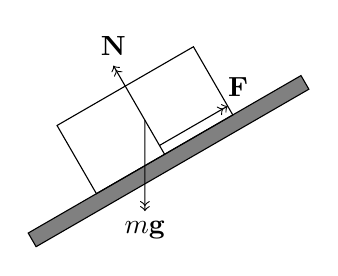
\begin{tikzpicture}[rotate = 30]
      \draw [fill=gray] (-2, 0) rectangle (2, -0.2);
      \draw (-1, 1) rectangle (1, 0);
      \draw [->>] (0, 0) -- (0, 1.3) node [above] {$\mathbf{N}$};
      \draw [->>] (0, 0.13) -- (1, 0.13) node [anchor = south west] {$\!\!\mathbf{F}$};
      \draw [->>] (0, 0.5) -- (-0.577, -0.5) node [below] {$m\mathbf{g}$};
    \end{tikzpicture}
\end{center}

\begin{definition}
    The friction is called \textbf{static friction} if no sliding occurs between surfaces.
\end{definition}

If static friction is exerted, $\bfF$ obeys 
\[
    |\bfF|\le \mu_s|\bfN|,
\]
where $\mu_s$ is called the \textbf{coefficient of static friction}. Block can remain static provided $ \alpha\le \arctan \mu_s $, where $ \alpha $ is the angle relative to the ground.

\begin{definition}
    If the block starts to slide, there is a \textbf{kinetic friction}.
\end{definition}
Here
\[
    |\bfF| = \mu_k|\bfN|
\]
where $ \mu_k $ is the \textbf{coefficient of kinetic friction}. In general, $ \mu_s>\mu_k>0 $, and their values depend on materials in contact. e.g. $ \mu_s\approx \mu_k\approx 0.8 $ between rubber and asphalt, and between teflons $ \mu_s\approx \mu_k\approx 0.04 $.

\subsubsection*{Fluid drag}
This happens when a solid body moves through a fluid. There are two important regimes for drag:
\begin{enumerate}[align=left]
    \item[\textbf{Linear drag}.] This happens when `small' objects moving through \textit{viscous} fluid, e.g. bacteria moving in body fluid. We have 
    \[
        \mathbf{F} = -k_1\bfu.
    \]
    If this object is a sphere with radius $R$, then \textit{Stokes force law} tells us that
    \[
        k_1 = 6\pi \eta R
    \]
    where $\eta$ is the viscosity of the fluid.
    \item[\textbf{Quadratic drag}.] This happens when large bodies are moving through less viscous fluids, e.g. a large fish swimming in water, cars, aircrafts, etc. We have 
    \[
        \mathbf{F} = -k_2 |\bfu|\bfu.
    \]
    Typically $k_2$ is given by 
    \[
        k_2 = \rho_{\text{fluid}}C_{\text{drag}}R^2,
    \]
    where $ \rho $ is the fluid density, $C$ is the drag coefficient, and $R$ is the size scale of the object.
\end{enumerate}

A body loses kinetic energy as a result of a drag force. Rates of working are 
\begin{align*}
    \bfF\cdot\bfu &= -k_1|\bfu|^2\quad \text{linear drag,}\\
    &= -k_2|\bfu|^3\quad \text{quadratic drag.} 
\end{align*}
In latter total work done $ \propto |\bfu|^2\cdot x $. The fluid gains energy as a result of drags.

\begin{example}
    Damped oscillator met in DEs. We have $ m \ddot{x} = -kx - \lambda \dot{x} $.
\end{example}
\begin{example}
    Consider a projectile moving under a uniform gravity and experiencing linear drag force.
    \[
        m \ddot{\bfx} = m\bfg -k \dot{\bfx},
    \]
    with initial conditions given by $ \bfx(0) = 0 $ and $ \dot{\bfx}(0)=\bfu_0 $. Solve for $ \dot{\bfx} $:
    \[
        \frac{\mathrm{d}}{\mathrm{d}t} (\dot{\bfx} e^{kt/m})=mge^{kt/m} \Longrightarrow \dot{\bfx} = \frac{m\bfg}{k}+\bfC e^{-kt/m} = \frac{m\bfg}{k}+\left( \bfu_0-\frac{m\bfg}{k} \right)e^{-kt/m}.
    \]
    Hence 
    \[
        \bfx = \frac{m\bfg}{k}t+\frac{m}{k}\left( \bfu_0-\frac{m\bfg}{k} \right)(1-e^{-kt/m}).
    \]
    Now consider components:
    \[
        \bfx=(x,y,z),\quad \bfu= (\bfu_1,\bfu_2,\bfu_3).
    \]
    Choose
    \[
        \bfu_0 = (u_0 \cos \theta,0,u_0 \sin \theta),\quad \bfg = (0,0,-g),
    \]
    then
    \begin{align*}
        u_1 &= u_0 \cos \theta e^{-kt/m},\\ 
        u_2 &= 0,\\
        u_3 &= \left( u_0\sin \theta+\frac{mg}{k} \right)e^{-kt/m}-\frac{mg}{k}.
    \end{align*}
    We see that $ u_1,u_2\to 0,u_3\to -\frac{mg}{k} $, so the \textbf{terminal velocity} is $ (0,0,-mg/k) $. This is achieved on a time scale $ m/k $. We also have 
    \begin{align*}
        x&= m u_0\frac{\cos \theta}{k}(1-e^{-kt/m}),\\ 
        y&= 0,\\ 
        z&= -\frac{mgt}{k}+\frac{m}{k}\left( u_0 \sin \theta+\frac{mg}{k} \right)(1-e^{-kt/m}).
    \end{align*}

    Now consider the \textbf{range} of the projectile: $x$ when $z$ returns to 0. We see that 
    \[
        R = R(u_0,\theta,m,k,g).
    \]
    Note that we can form a \textit{dimensionless group} such that 
    \[
        \frac{ku_0}{mg} = \frac{u_0/g}{m/k},
    \]
    where $u_0/g$ is time taken to reduce initial velocity by gravity, and $m/k$ is the time taken to achieve terminal velocity. Dimensional analysis gives 
    \[
        R = \frac{u_0^2}{g}F\left( \theta,\frac{ku_0}{mg} \right).
    \] 
    When the friction is weak, $ ku_0/mg\ll 1 $ and $ R = \frac{2u_0^2}{g}\sin \theta \cos \theta  $. When the friction is large, $ ku_0/mg\gg 1 $ and $ R=\frac{U^2}{g}\left( \frac{mg}{ku_0}\cos \theta \right) $.
\end{example}
The lecturer talked quite badly about this example and \href{http://www.damtp.cam.ac.uk/user/tong/relativity/two.pdf\#page=27}{this page} gives a better illustration.